\section{Behistun Inscription}

\begin{figure}[H]
    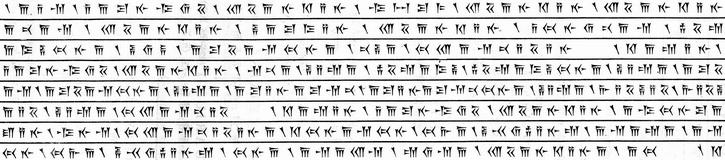
\includegraphics[width=\textwidth]{column-i-lines-1-8}
    \caption{Behistun Inscription, Column i, lines 1-8\cite{BehistunT01}}
\end{figure}

\begin{enumerate}
    \item {\oldpersian ;}\stackunder{{\oldpersian adm}}{(Pronoun) I\cite{adm}} {\oldpersian ;} \stackunder{{\oldpersian daryvuS}}{Darius\textsuperscript{\cite[p185]{rawlinson1849memoir}}\cite{darius}}{\oldpersian ;} \stackunder{\oldpersian xsayoiy}{Alternative form of {\oldpersian Q}\cite{alternativeKing}} {\oldpersian ;} {\oldpersian vzrk}
\end{enumerate}

\begin{enumerate}
    \item I am Darius, the great king, king of kings, the king of Persia, the king of countries, the son of Hystaspes,
         the grandson of Arsames, the Achaemenid.
    \item King Darius says: My father is Hystaspes; the father of Hystaspes was Arsames; the father of Arsames was
          Ariaramnes; the father of Ariaramnes was Teispes; the father of Teispes was Achaemenes.
    \item King Darius says: That is why we are called Achaemenids; from antiquity we have been noble; from antiquity
          has our dynasty been royal.
\end{enumerate}
